\documentclass[conference]{IEEEtran}

\usepackage[utf8]{inputenc}
\usepackage[T1]{fontenc}
\usepackage[brazil]{babel}
\usepackage{placeins}
\usepackage{cite}
\usepackage{graphicx}
\usepackage{url}
\usepackage{amsmath}
\usepackage{booktabs}
\usepackage{multirow}
\usepackage{float}
\usepackage{capt-of}

% Ajustes para melhor controle de floats em duas colunas
\renewcommand{\topfraction}{0.9}
\renewcommand{\bottomfraction}{0.8}
\renewcommand{\textfraction}{0.07}
\renewcommand{\floatpagefraction}{0.7}
\setcounter{topnumber}{4}
\setcounter{bottomnumber}{4}
\setcounter{totalnumber}{6}

\begin{document}

\title{Predi\c{c}\~ao de Diabetes Mellitus Tipo 2 Utilizando T\'{e}cnicas de Intelig\^{e}ncia Computacional: Uma An\'{a}lise Comparativa}

\author{
\IEEEauthorblockN{Rafael A. S. Ferreira}
\IEEEauthorblockA{\textit{Engenharia da Computa\c{c}\~ao} \\
\textit{CEFET-MG Campus V}\\
Divin\'{o}polis, Brasil \\
rafael.ferreira@aluno.cefetmg.br}
\and
\IEEEauthorblockN{Jo\~ao M. G. Lisboa}
\IEEEauthorblockA{\textit{Engenharia da Computa\c{c}\~ao} \\
\textit{CEFET-MG Campus V}\\
Divin\'{o}polis, Brasil \\
joao.lisboa@aluno.cefetmg.br}
\and
\IEEEauthorblockN{Gabriel V. Silva}
\IEEEauthorblockA{\textit{Engenharia da Computa\c{c}\~ao} \\
\textit{CEFET-MG Campus V}\\
Divin\'{o}polis, Brasil \\
gabriel.silva@aluno.cefetmg.br}
}

\maketitle

\begin{abstract}
O Diabetes Mellitus Tipo 2 (DMT2) \'{e} um dos principais desafios de sa\'{u}de p\'{u}blica contempor\^{a}neos, afetando mais de 537 milh\~oes de adultos mundialmente. A identifica\c{c}\~ao precoce de indiv\'{i}duos em risco \'{e} fundamental para a preven\c{c}\~ao de complica\c{c}\~oes e redu\c{c}\~ao de custos hospitalares. Este trabalho conduz uma an\'{a}lise comparativa de quatro t\'{e}cnicas de Intelig\^{e}ncia Computacional aplicadas \`{a} predi\c{c}\~ao de diabetes: Multi-Layer Perceptron (MLP), Support Vector Machine (SVM), Random Forest (RF) e Regress\~ao Log\'{i}stica. Utilizando o dataset PIMA Indians Diabetes, aplicamos um pipeline rigoroso de pr\'{e}-processamento, incluindo tratamento de zeros imposs\'{i}veis, imputa\c{c}\~ao por mediana, padroniza\c{c}\~ao e balanceamento via SMOTE. A sele\c{c}\~ao de hiperpar\^{a}metros foi realizada por GridSearchCV com valida\c{c}\~ao cruzada de 5 folds. Os resultados demonstram que a Regress\~ao Log\'{i}stica obteve o melhor desempenho geral, com F1-Score de 0,656 e AUC-ROC de 0,814 no conjunto de teste, seguida pelo MLP (F1=0,623; AUC=0,812). Todos os modelos alcan\c{c}aram AUC-ROC superior a 0,79, indicando capacidade discriminativa satisfat\'{o}ria. Os resultados evidenciam que modelos mais simples podem superar arquiteturas complexas em bases de pequeno porte.
\end{abstract}

\begin{IEEEkeywords}
Diabetes Mellitus Tipo 2, Intelig\^{e}ncia Computacional, Aprendizado de M\'{a}quina, Multi-Layer Perceptron, Support Vector Machine, Random Forest, Regress\~ao Log\'{i}stica.
\end{IEEEkeywords}

\section{Introdu\c{c}\~ao}

O Diabetes Mellitus Tipo 2 (DMT2) configura-se como uma das epidemias de sa\'{u}de mais significativas do s\'{e}culo XXI. Segundo o 10º Atlas da Diabetes da Federa\c{c}\~ao Internacional de Diabetes (IDF), aproximadamente 537 milh\~oes de adultos entre 20 e 79 anos viviam com a doen\c{c}a em 2021, com proje\c{c}\~ao de crescimento para 783 milh\~oes at\'{e} 2045~\cite{idf2021}. O Brasil ocupa a 6ª posi\c{c}\~ao no ranking mundial de preval\^{e}ncia, com cerca de 16,8 milh\~oes de indiv\'{i}duos afetados~\cite{idf2021}.

A natureza progressiva e frequentemente silenciosa do DMT2 torna o diagn\'{o}stico tardio um problema recorrente. Estudos indicam que at\'{e} 50\% dos casos permanecem n\~ao diagnosticados por anos, per\'{i}odo durante o qual complica\c{c}\~oes micro e macrovasculares j\'{a} se instalam~\cite{kavakiotis2017}. A capacidade de predizer o risco de diabetes com anteced\^{e}ncia, a partir de exames cl\'{i}nicos rotineiros, representa uma oportunidade transformadora para a medicina preventiva.

Nesse contexto, as t\'{e}cnicas de Intelig\^{e}ncia Computacional (IC) emergem como ferramentas particularmente adequadas. A rela\c{c}\~ao entre fatores de risco e desenvolvimento do diabetes \'{e} intrinsecamente n\~ao-linear e multivariada~\cite{haykin2009}. Algoritmos de Aprendizado de M\'{a}quina s\~ao capazes de capturar padr\~oes sutis em dados cl\'{i}nicos sem a necessidade de modelagem expl\'{i}cita das rela\c{c}\~oes entre vari\'{a}veis.

O objetivo deste trabalho \'{e} realizar uma an\'{a}lise comparativa sistem\'{a}tica de quatro algoritmos de AM para predi\c{c}\~ao de DMT2: MLP, SVM, Random Forest e Regress\~ao Log\'{i}stica. A contribui\c{c}\~ao principal reside na avalia\c{c}\~ao rigorosa sob condi\c{c}\~oes experimentais uniformes, incluindo busca exaustiva de hiperpar\^{a}metros via GridSearchCV, balanceamento de classes com SMOTE e m\'{e}tricas apropriadas para dados desbalanceados.

\section{Revis\~ao da Literatura}

A aplica\c{c}\~ao de t\'{e}cnicas de IC na predi\c{c}\~ao e manejo do diabetes tem crescido substancialmente nas \'{u}ltimas duas d\'{e}cadas. Smith et al.~\cite{smith1988} estabeleceram uma das bases mais importantes ao disponibilizar o PIMA Indians Diabetes Dataset, composto por dados cl\'{i}nicos de mulheres da tribo Pima, no Arizona. Esse conjunto tornou-se refer\^{e}ncia para benchmarking de algoritmos de AM em problemas de sa\'{u}de.

Sisodia e Sisodia~\cite{sisodia2018} conduziram um estudo comparativo utilizando Naive Bayes, k-NN e SVM no dataset PIMA, alcan\c{c}ando acur\'{a}cia m\'{a}xima de aproximadamente 77\% com Naive Bayes. Maniruzzaman et al.~\cite{maniruzzaman2017} expandiram essa an\'{a}lise incorporando SVM com kernel RBF e Random Forest, demonstrando que esses m\'{e}todos superam abordagens lineares quando adequadamente parametrizados. Kaur e Kumari~\cite{kaur2021} apresentaram uma revis\~ao sistem\'{a}tica de 45 trabalhos e constataram que ensembles baseados em \'{a}rvores consistentemente figuram entre os melhores desempenhos.

Apesar da quantidade crescente de trabalhos, observa-se uma lacuna: a maioria dos estudos n\~ao realiza compara\c{c}\~oes sistem\'{a}ticas com busca exaustiva de hiperpar\^{a}metros nem emprega t\'{e}cnicas de balanceamento de forma consistente. Adicionalmente, poucos avaliam o desempenho por meio de m\'{e}tricas adequadas para dados desbalanceados, como F1-Score e AUC-ROC. Este trabalho visa preencher parcialmente essa lacuna.

\section{Materiais e M\'{e}todos}

\subsection{Descri\c{c}\~ao dos Dados}

Este estudo utiliza o PIMA Indians Diabetes Database, disponibilizado pelo UCI Machine Learning Repository~\cite{smith1988,uci2024}. O dataset cont\'{e}m 768 amostras coletadas de mulheres da tribo Pima Indian, com idade igual ou superior a 21 anos. Cada amostra possui 8 atributos num\'{e}ricos preditivos e 1 vari\'{a}vel alvo bin\'{a}ria, conforme a Tabela~\ref{tab:atributos}.

\begin{table}[H]
\caption{Descri\c{c}\~ao dos atributos do dataset PIMA Indians Diabetes.}
\label{tab:atributos}
\centering
\scriptsize
\setlength{\tabcolsep}{2pt}
\begin{tabular}{@{}llcc@{}}
\toprule
Atributo & Descri\c{c}\~ao & Tipo & Faixa T\'{i}pica \\
\midrule
NumGestacoes & N\'{u}mero de gesta\c{c}\~oes & Num\'{e}rico & 0 -- 17 \\
Glicose & Concentra\c{c}\~ao plasm\'{a}tica de glicose & Num\'{e}rico & 0 -- 199 mg/dL \\
Press\~aoArterial & Press\~ao arterial diast\'{o}lica & Num\'{e}rico & 0 -- 122 mmHg \\
EspessuraPele & Espessura da dobra cut\^{a}nea do tr\'{i}ceps & Num\'{e}rico & 0 -- 99 mm \\
Insulina & N\'{i}vel de insulina s\'{e}rica & Num\'{e}rico & 0 -- 846 mu U/mL \\
IMC & \'{I}ndice de Massa Corporal & Num\'{e}rico & 0 -- 67,1 kg/m$^2$ \\
Pedigree & Fun\c{c}\~ao pedigree de diabetes & Num\'{e}rico & 0,078 -- 2,42 \\
Idade & Idade em anos & Num\'{e}rico & 21 -- 81 \\
\textbf{Alvo: Diabetes} & \textbf{Presen\c{c}a de DMT2} & \textbf{Bin\'{a}rio} & \textbf{0 / 1} \\
\bottomrule
\end{tabular}
\end{table}

O dataset apresenta desbalanceamento entre as classes: 500 inst\^{a}ncias (65,1\%) da classe negativa e 268 inst\^{a}ncias (34,9\%) da classe positiva. Adicionalmente, cinco atributos biol\'{o}gicos apresentam valores zero fisicamente imposs\'{i}veis: Glicose (5 zeros), Press\~ao Arterial (35), Espessura da Pele (227), Insulina (374) e IMC (11). Esses valores foram interpretados como dados faltantes codificados.

\subsection{An\'{a}lise Explorat\'{o}ria}

A an\'{a}lise explorat\'{o}ria inicial revelou as principais caracter\'{i}sticas do dataset. A Figura~\ref{fig:correlacao} apresenta o mapa de correla\c{c}\~ao entre os atributos. Observa-se que \textbf{Glicose} e \textbf{IMC} s\~ao as vari\'{a}veis com maior correla\c{c}\~ao positiva com a presen\c{c}a de diabetes, o que \'{e} clinicamente esperado, j\'{a} que ambos s\~ao fatores de risco bem estabelecidos para o DMT2. A vari\'{a}vel \textbf{Idade} tamb\'{e}m apresenta correla\c{c}\~ao moderada com o alvo, enquanto atributos como \textbf{Espessura da Pele} e \textbf{Press\~ao Arterial} mostram correla\c{c}\~oes mais fracas. A alta propor\c{c}\~ao de zeros nas vari\'{a}veis Insulina e Espessura da Pele evidencia a necessidade do tratamento de dados faltantes codificados.

\begin{figure}[H]
    \centering
    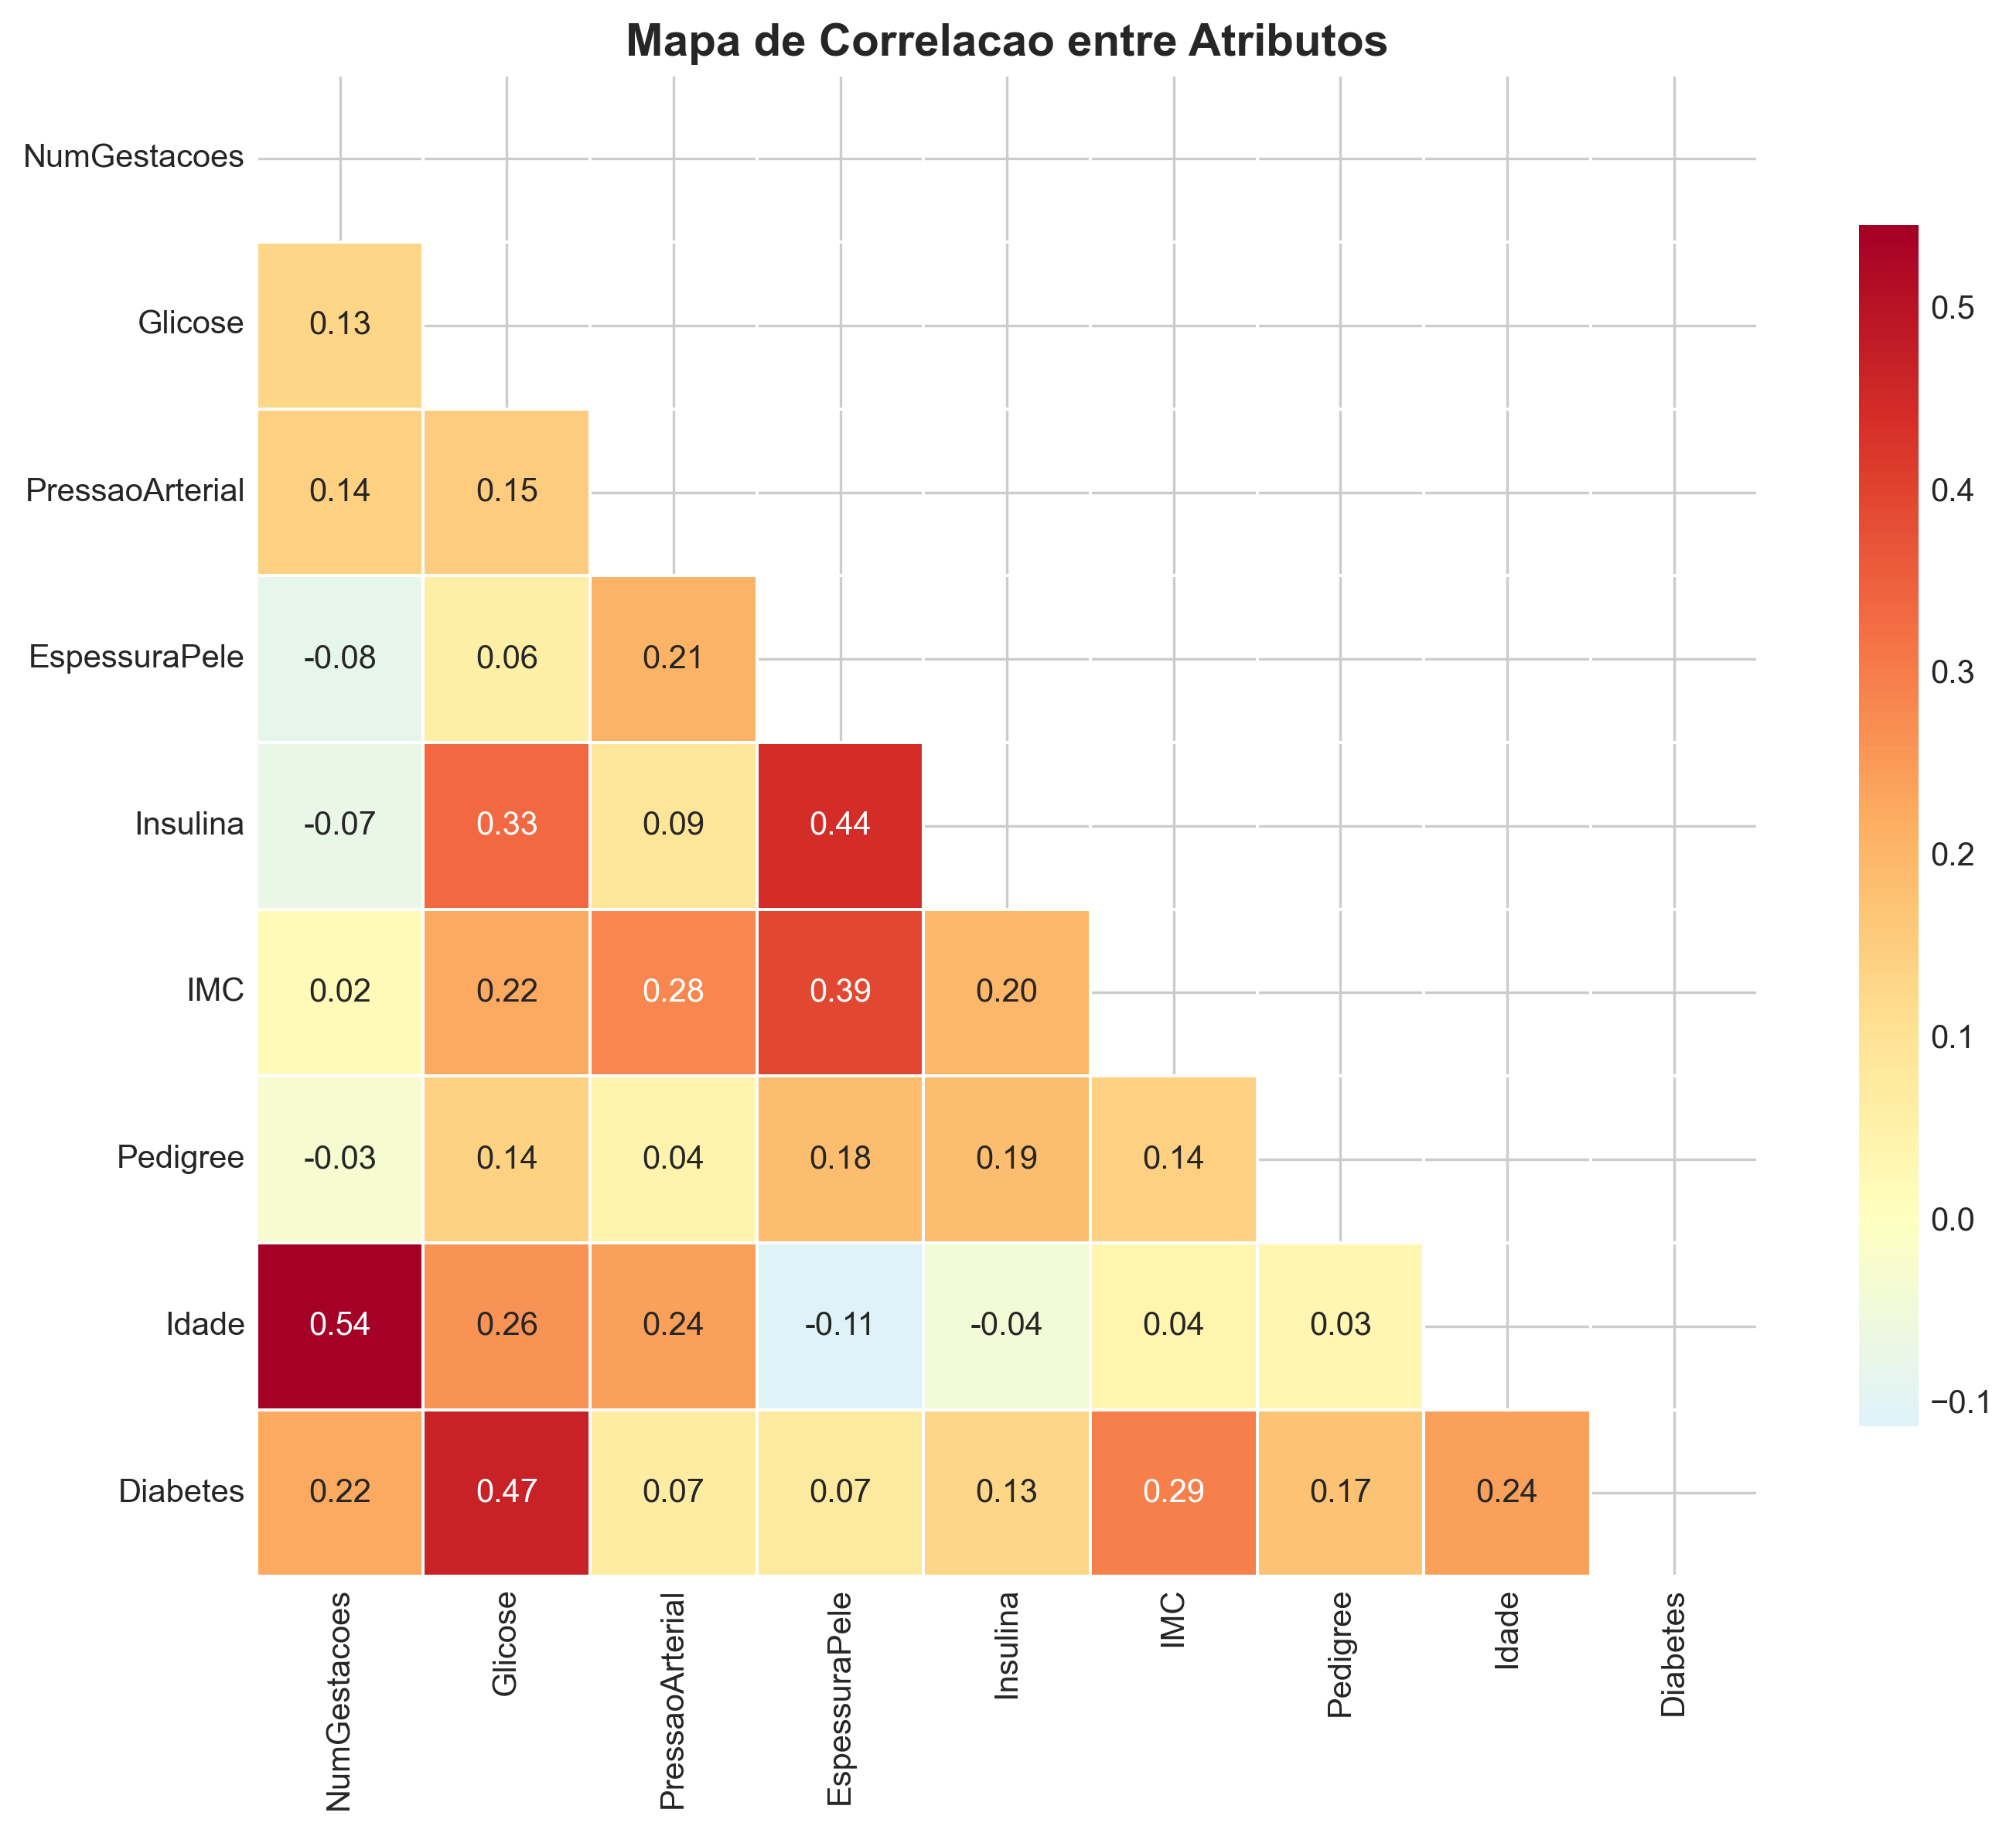
\includegraphics[width=0.95\linewidth]{figuras_diabetes/01_correlacao.png}
    \caption{Mapa de correla\c{c}\~ao entre os atributos do dataset PIMA Indians Diabetes.}
    \label{fig:correlacao}
\end{figure}

\subsection{Pr\'{e}-processamento}

O pipeline de pr\'{e}-processamento foi executado na seguinte sequ\^{e}ncia: \textbf{(a)} zeros imposs\'{i}veis foram substitu\'{i}dos por NaN; \textbf{(b)} valores faltantes foram imputados pela mediana calculada no conjunto de treino; \textbf{(c)} os dados foram divididos de forma estratificada em 60\% treino (460 amostras), 20\% valida\c{c}\~ao (154) e 20\% teste (154), com \texttt{random\_state=42}; \textbf{(d)} aplicou-se \texttt{StandardScaler} ajustado apenas no treino; e \textbf{(e)} utilizou-se SMOTE exclusivamente no conjunto de treino, balanceando as classes de 300/160 para 300/300 amostras.

\subsection{Algoritmos Avaliados}

Foram avaliados quatro algoritmos de classifica\c{c}\~ao, representando paradigmas distintos:

\textbf{MLP} -- rede neural feedforward treinada por backpropagation, capaz de aproximar fun\c{c}\~oes universais e capturar rela\c{c}\~oes n\~ao-lineares complexas~\cite{haykin2009}.

\textbf{SVM} -- classificador que busca o hiperplano de separa\c{c}\~ao \'{o}timo maximizando a margem entre classes. Atrav\'{e}s do \textit{kernel trick}, projeta os dados para espa\c{c}os de maior dimensionalidade.

\textbf{Random Forest} -- m\'{e}todo de ensemble baseado em \textit{bagging} de m\'{u}ltiplas \'{a}rvores de decis\~ao, conferindo robustez contra overfitting e fornecendo estimativas de import\^{a}ncia de vari\'{a}veis.

\textbf{Regress\~ao Log\'{i}stica} -- modelo linear generalizado altamente interpret\'{a}vel, que estima probabilidades via fun\c{c}\~ao log\'{i}stica e possui regulariza\c{c}\~ao integrada.

\subsection{Configura\c{c}\~ao dos Par\^{a}metros}

A sele\c{c}\~ao de hiperpar\^{a}metros foi realizada por \texttt{GridSearchCV} com valida\c{c}\~ao cruzada de 5 folds, utilizando F1-Score como m\'{e}trica de otimiza\c{c}\~ao. Os espa\c{c}os de busca definidos s\~ao apresentados a seguir.

\textbf{MLP:} \texttt{hidden\_layer\_sizes} [(16,8), (32,16), (64,32)], \texttt{activation} [relu, tanh], \texttt{learning\_rate\_init} [0,001, 0,01], \texttt{max\_iter} [500], \texttt{early\_stopping} [True].

\textbf{SVM:} \texttt{C} [0,1, 1, 10, 100], \texttt{kernel} [rbf, linear], \texttt{gamma} [scale, auto].

\textbf{RF:} \texttt{n\_estimators} [50, 100, 200], \texttt{max\_depth} [None, 10, 20], \texttt{min\_samples\_split} [2, 5].

\textbf{Regress\~ao Log\'{i}stica:} \texttt{C} [0,01, 0,1, 1, 10], \texttt{solver} [liblinear, lbfgs].

Os melhores par\^{a}metros encontrados s\~ao apresentados na Tabela~\ref{tab:parametros}.

\begin{table}[H]
\caption{Melhores par\^{a}metros encontrados via GridSearchCV.}
\label{tab:parametros}
\centering
\scriptsize
\setlength{\tabcolsep}{2pt}
\begin{tabular}{@{}lp{4.8cm}c@{}}
\toprule
Modelo & Melhores Par\^{a}metros & F1 (CV) \\
\midrule
MLP & activation=relu, hidden\_layer\_sizes=(64,32), lr=0,01 & 0,778 \\
SVM & C=100, kernel=rbf, gamma=auto & 0,793 \\
RF & n\_estimators=50, max\_depth=None, min\_samples\_split=2 & 0,822 \\
LogReg & C=1, solver=liblinear & 0,757 \\
\bottomrule
\end{tabular}
\end{table}

\subsection{Procedimento Experimental}

Todos os algoritmos foram avaliados sob as \textbf{mesmas condi\c{c}\~oes experimentais}: mesma parti\c{c}\~ao estratificada dos dados, mesmo pipeline de pr\'{e}-processamento e mesmas m\'{e}tricas de avalia\c{c}\~ao. A divis\~ao em treino, valida\c{c}\~ao e teste foi realizada uma \'{u}nica vez e reproduzida de forma id\^{e}ntica para todos os modelos, garantindo uma compara\c{c}\~ao justa entre as abordagens.

O \texttt{GridSearchCV} foi executado exclusivamente sobre o conjunto de treino (ap\'{o}s o SMOTE), utilizando valida\c{c}\~ao cruzada de 5 folds para sele\c{c}\~ao dos hiperpar\^{a}metros. O conjunto de valida\c{c}\~ao (20\%) foi reservado para aferi\c{c}\~ao final dos modelos candidatos durante a busca em grade. Por fim, o conjunto de \textbf{teste foi utilizado apenas uma \'{u}nica vez para a avalia\c{c}\~ao final}, sem influenciar qualquer etapa de treinamento, valida\c{c}\~ao ou sele\c{c}\~ao de hiperpar\^{a}metros. Essa pr\'{a}tica evita vazamento de informa\c{c}\~ao (data leakage) e assegura que as m\'{e}tricas reportadas reflitam a capacidade de generaliza\c{c}\~ao real dos modelos.

\subsection{M\'{e}tricas de Avalia\c{c}\~ao}

Considerando o desbalanceamento das classes, foram empregadas: acur\'{a}cia, precis\~ao, revoca\c{c}\~ao, F1-Score e AUC-ROC. Modelos estoc\'{a}sticos (MLP e RF) foram executados 10 vezes com diferentes sementes aleat\'{o}rias, reportando m\'{e}dia $\pm$ desvio-padr\~ao. SVM e Regress\~ao Log\'{i}stica, por serem determin\'{i}sticos, foram executados uma \'{u}nica vez.

\section{Resultados e Discuss\~ao}

\subsection{Desempenho dos Modelos}

A Tabela~\ref{tab:resultados} apresenta os resultados obtidos no conjunto de teste. A Regress\~ao Log\'{i}stica obteve o melhor F1-Score (0,656) e AUC-ROC (0,814), seguida pelo MLP (F1=0,623; AUC=0,812). Todos os modelos alcan\c{c}aram AUC-ROC superior a 0,79.

\begin{table}[H]
\caption{Resultados de desempenho no conjunto de teste (m\'{e}dia $\pm$ desvio-padr\~ao, N=10).}
\label{tab:resultados}
\centering
\scriptsize
\setlength{\tabcolsep}{1.5pt}
\begin{tabular}{@{}lccccc@{}}
\toprule
Modelo & Acur\'{a}cia & Precis\~ao & Revoca\c{c}\~ao & F1-Score & AUC-ROC \\
\midrule
MLP & 0,718 $\pm$ 0,012 & 0,587 $\pm$ 0,017 & 0,667 $\pm$ 0,050 & 0,623 $\pm$ 0,023 & 0,812 $\pm$ 0,007 \\
SVM & 0,721 & 0,604 & 0,593 & 0,598 & 0,792 \\
RF & 0,733 $\pm$ 0,012 & 0,619 $\pm$ 0,016 & 0,622 $\pm$ 0,026 & 0,620 $\pm$ 0,020 & 0,808 $\pm$ 0,004 \\
LogReg & \textbf{0,734} & 0,600 & \textbf{0,722} & \textbf{0,656} & \textbf{0,814} \\
\bottomrule
\end{tabular}
\end{table}

A Tabela~\ref{tab:confusao} apresenta as matrizes de confus\~ao consolidadas no conjunto de teste. A Regress\~ao Log\'{i}stica apresentou o maior n\'{u}mero de verdadeiros positivos (39) e o menor de falsos negativos (15), confirmando sua superioridade em identificar corretamente pacientes diab\'{e}ticos.

\begin{table}[H]
\caption{Matriz de confus\~ao no conjunto de teste.}
\label{tab:confusao}
\centering
\scriptsize
\setlength{\tabcolsep}{4pt}
\begin{tabular}{@{}lcccc@{}}
\toprule
Modelo & VP & VN & FP & FN \\
\midrule
MLP & 40 & 73 & 27 & 14 \\
SVM & 32 & 79 & 21 & 22 \\
RF & 32 & 80 & 20 & 22 \\
LogReg & 39 & 74 & 26 & 15 \\
\bottomrule
\end{tabular}
\end{table}

\subsection{Impacto dos Hiperpar\^{a}metros}

A busca em grade revelou comportamentos importantes. O MLP obteve melhor desempenho com arquitetura moderada (64,32) e \texttt{learning\_rate\_init}=0,01, enquanto arquiteturas menores ou taxas de aprendizado mais baixas resultaram em menor F1 na valida\c{c}\~ao cruzada. O SVM selecionou \texttt{C}=100 e kernel RBF, indicando necessidade de fronteira de decis\~ao flex\'{i}vel; contudo, essa mesma flexibilidade pode ter causado overfitting no conjunto de teste. O Random Forest preferiu apenas 50 \'{a}rvores e profundidade ilimitada, sugerindo que o aumento do n\'{u}mero de \'{a}rvores n\~ao compensou a restri\c{c}\~ao imposta pelo pequeno dataset. A Regress\~ao Log\'{i}stica selecionou \texttt{C}=1, ponto intermedi\'{a}rio de regulariza\c{c}\~ao L2 que balanceou bem vi\'{e}s e vari\^{a}ncia.

\subsection{An\'{a}lise por Modelo}

A Regress\~ao Log\'{i}stica obteve desempenho superior apesar de sua simplicidade, o que pode ser atribu\'{i}do \`{a} escassez de dados (apenas 460 amostras de treino pr\'{e}-SMOTE), condi\c{c}\~ao em que modelos com menos par\^{a}metros tendem a generalizar melhor~\cite{russel2021}. Sua revoca\c{c}\~ao de 0,722 -- a mais alta entre os modelos -- \'{e} cr\'{i}tica em contextos de sa\'{u}de, onde falsos negativos t\^{e}m consequ\^{e}ncias mais graves.

O MLP obteve o segundo melhor F1-Score (0,623), com AUC-ROC competitivo (0,812). Contudo, apresentou a maior variabilidade entre execu\c{c}\~oes (desvio-padr\~ao de 0,023 no F1-Score), evidenciando sensibilidade \`{a} inicializa\c{c}\~ao aleat\'{o}ria dos pesos.

O Random Forest apresentou desempenho est\'{a}vel (menor desvio-padr\~ao entre os modelos estoc\'{a}sticos: 0,020 no F1-Score), mas limitado em magnitude. A an\'{a}lise de import\^{a}ncia de vari\'{a}veis revelou que Glicose e IMC s\~ao, por larga margem, os atributos mais discriminativos, resultado consistente com o conhecimento cl\'{i}nico.

O SVM obteve o menor F1-Score (0,598). Apesar da flexibilidade do kernel RBF, a alta regulariza\c{c}\~ao (C=100) combinada com o pequeno volume de treino pode ter levado a um modelo excessivamente flex\'{i}vel.

\subsection{Visualiza\c{c}\~ao dos Resultados}

A Figura~\ref{fig:roc} apresenta as curvas ROC dos modelos, destacando a capacidade discriminativa semelhante entre Regress\~ao Log\'{i}stica e MLP. A Figura~\ref{fig:metricas} compara as principais m\'{e}tricas, refor\c{c}ando a superioridade da Regress\~ao Log\'{i}stica no F1-Score. A Figura~\ref{fig:features} mostra a import\^{a}ncia relativa das vari\'{a}veis preditoras segundo o Random Forest.

\begin{figure}[H]
    \centering
    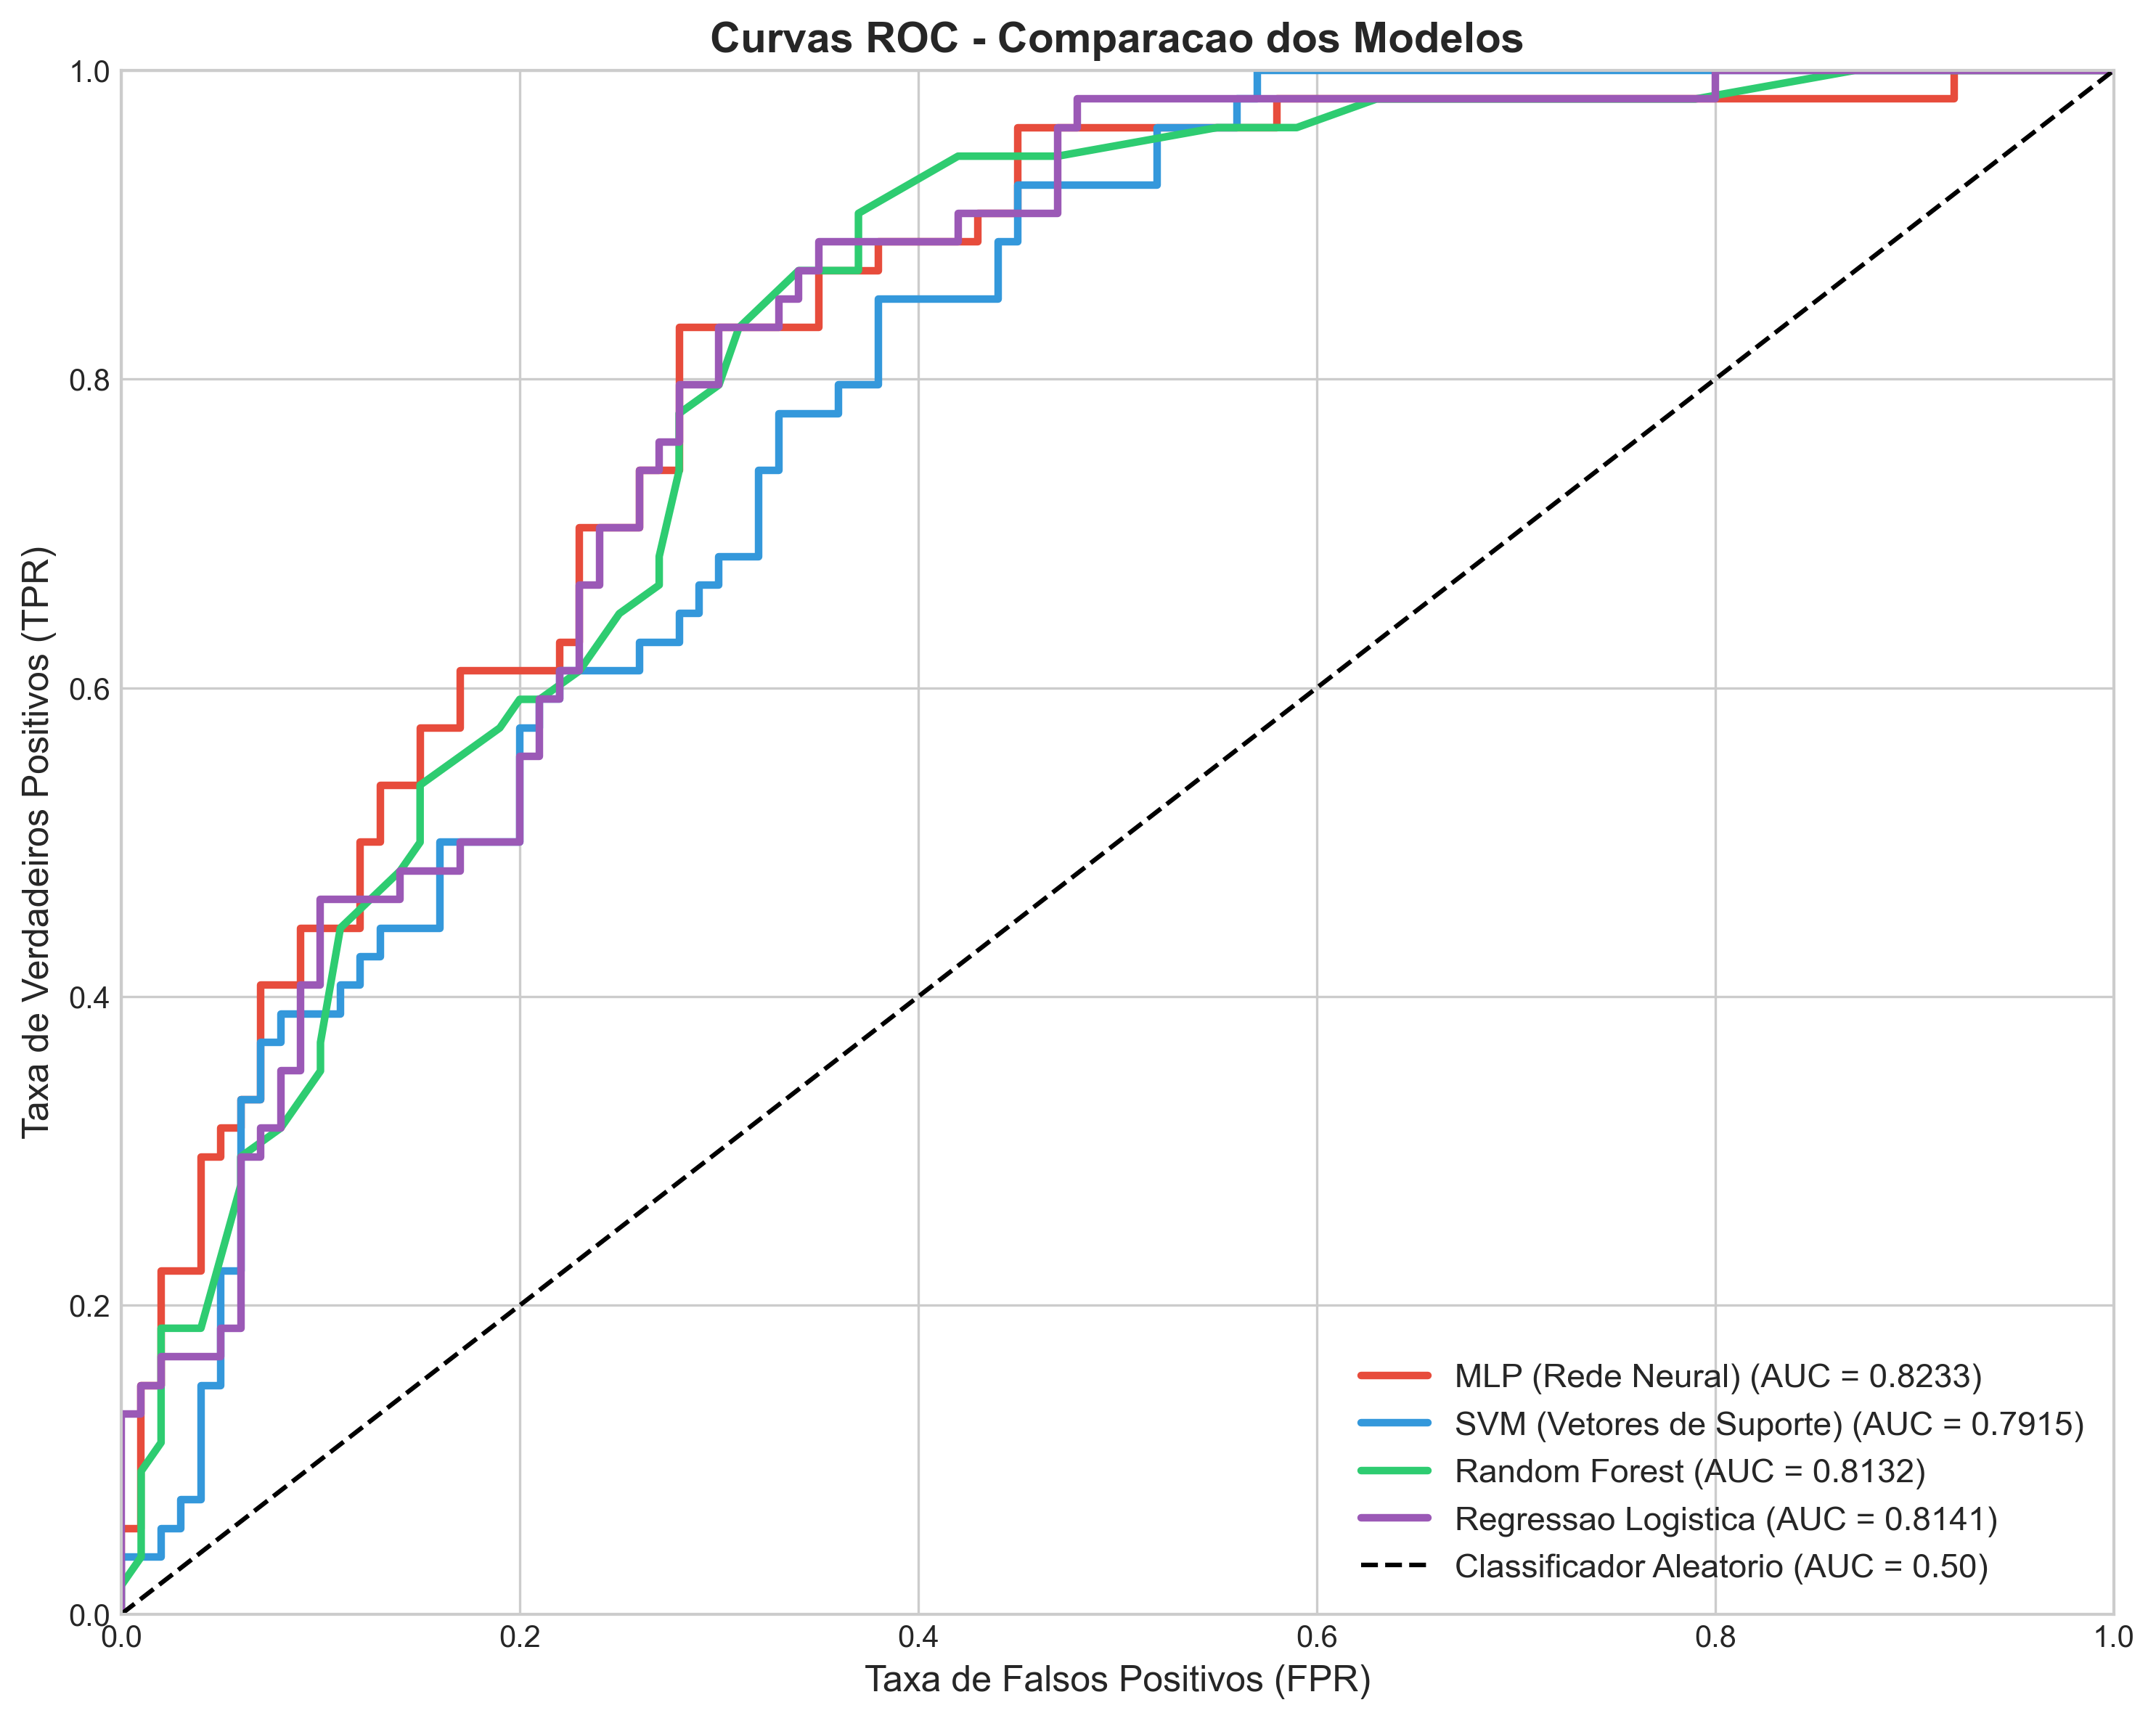
\includegraphics[width=0.95\linewidth]{figuras_diabetes/04_curvas_roc.png}
    \caption{Curvas ROC dos modelos no conjunto de teste.}
    \label{fig:roc}
\end{figure}

\begin{figure}[H]
    \centering
    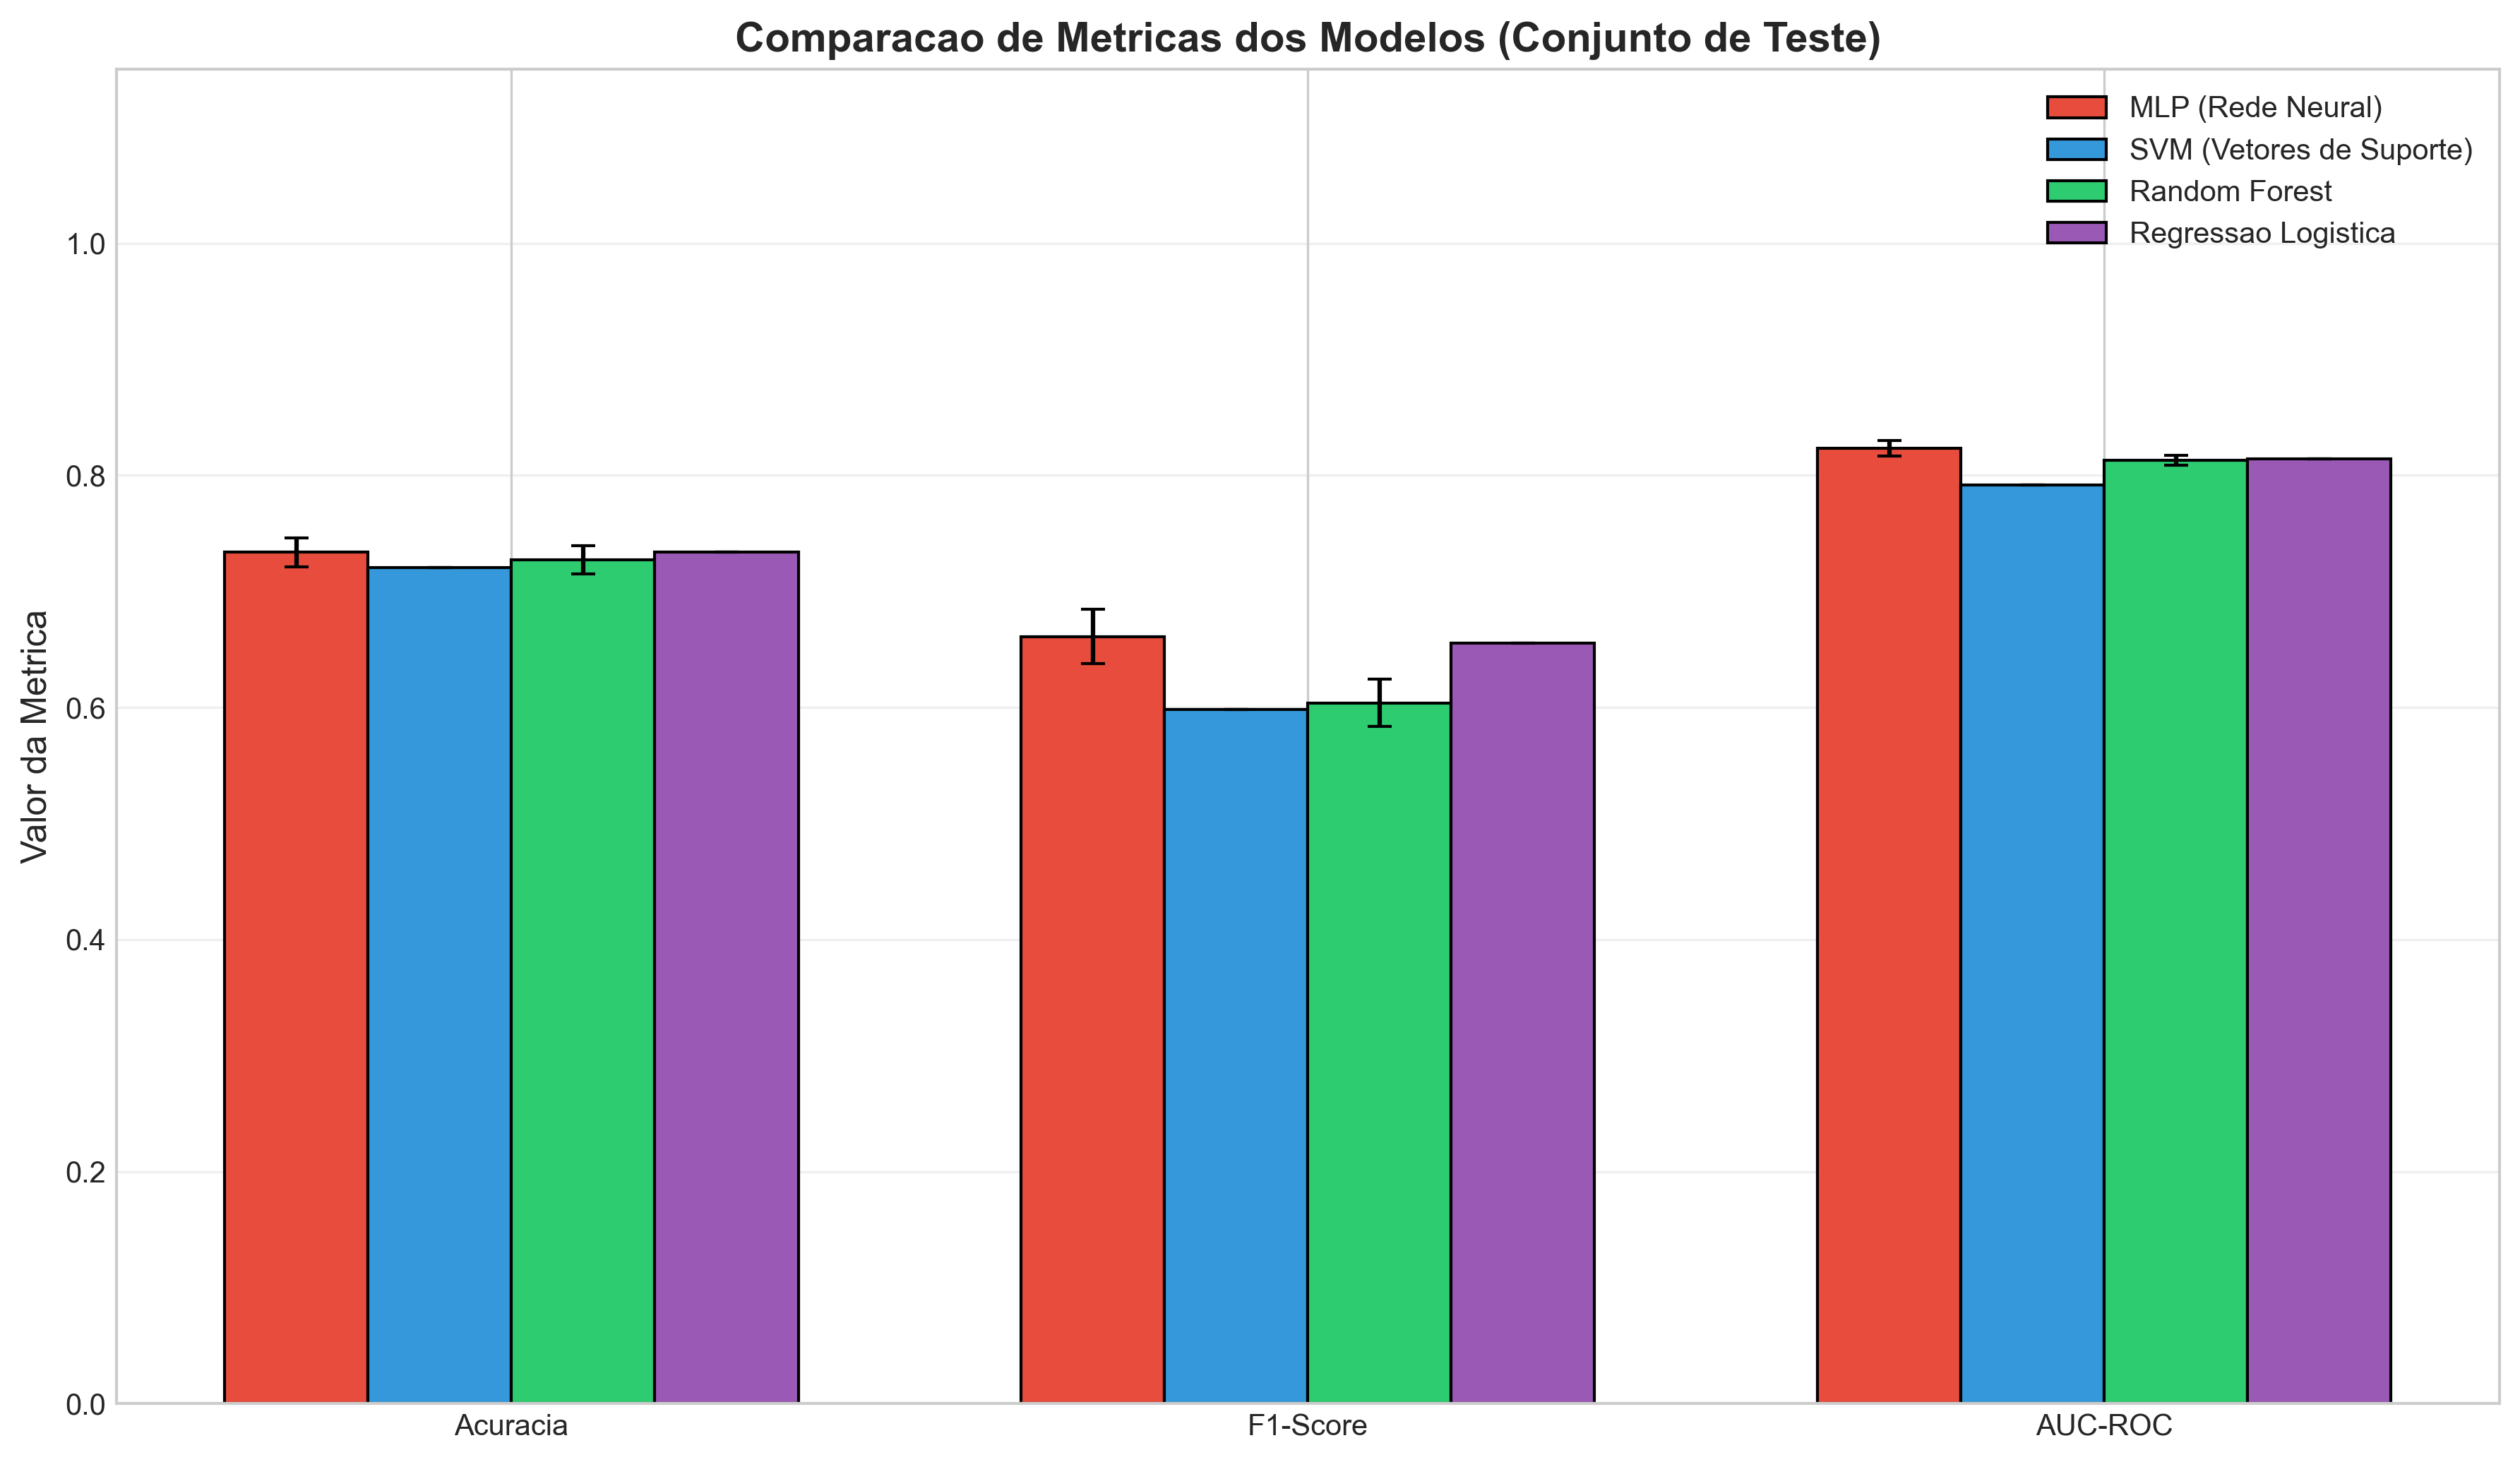
\includegraphics[width=0.95\linewidth]{figuras_diabetes/05_comparacao_metricas.png}
    \caption{Compara\c{c}\~ao de acur\'{a}cia, F1-Score e AUC-ROC.}
    \label{fig:metricas}
\end{figure}

\begin{figure}[H]
    \centering
    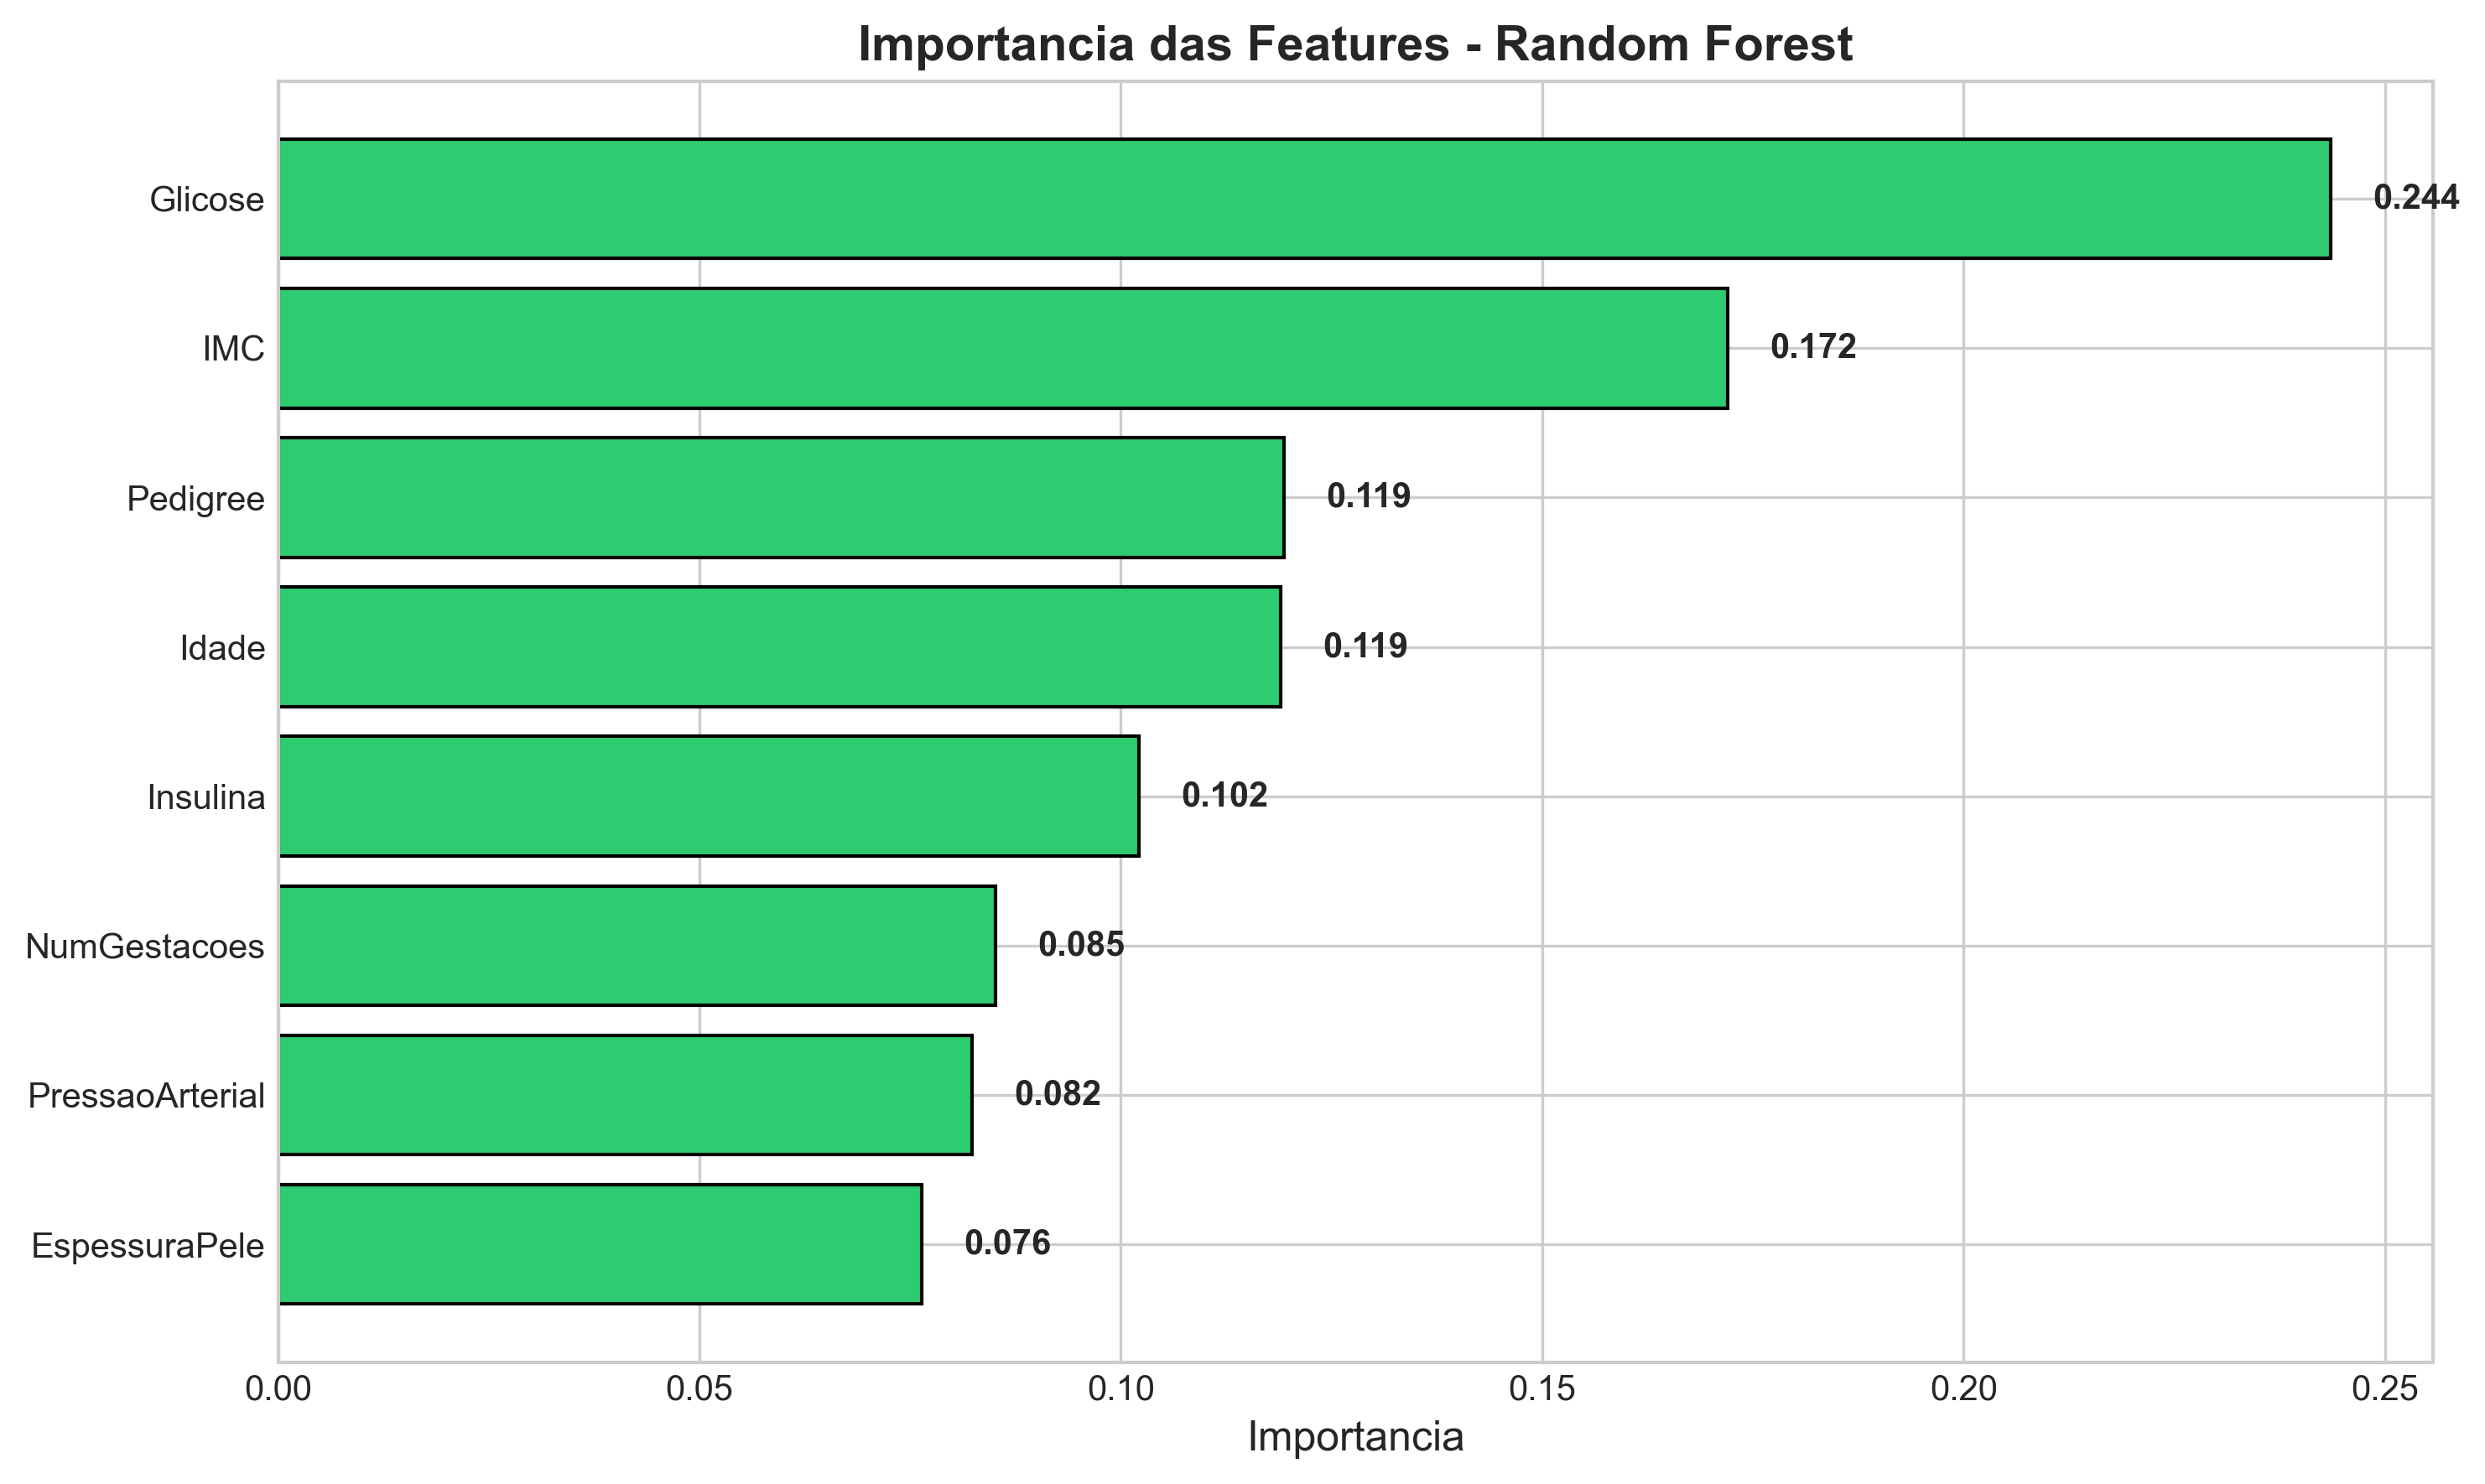
\includegraphics[width=0.95\linewidth]{figuras_diabetes/07_feature_importance.png}
    \caption{Import\^{a}ncia das vari\'{a}veis preditoras -- Random Forest.}
    \label{fig:features}
\end{figure}

\subsection{Discuss\~ao Geral}

Todos os modelos alcan\c{c}aram AUC-ROC superior a 0,79, indicando capacidade discriminativa satisfat\'{o}ria segundo os crit\'{e}rios de Hosmer e Lemeshow~\cite{hosmer2013}. O F1-Score relativamente modesto (0,598 a 0,656) reflete a dificuldade intr\'{i}nseca da predi\c{c}\~ao a partir de oito vari\'{a}veis cl\'{i}nicas, sem acesso a marcadores bioqu\'{i}micos mais espec\'{i}ficos.

A compara\c{c}\~ao com resultados reportados na literatura mostra consist\^{e}ncia. Sisodia e Sisodia~\cite{sisodia2018} reportaram acur\'{a}cia de aproximadamente 77\% com Naive Bayes no mesmo dataset, valor compar\'{a}vel \`{a} acur\'{a}cia de 73\% observada neste estudo. Maniruzzaman et al.~\cite{maniruzzaman2017} reportaram AUC-ROC entre 0,80 e 0,85 para SVM e Random Forest, faixa compat\'{i}vel com os nossos resultados.

O predom\'{i}nio da Regress\~ao Log\'{i}stica sobre abordagens mais sofisticadas refor\c{c}a o princ\'{i}pio de que a complexidade do modelo deve estar adequada \`{a} quantidade e qualidade dos dados dispon\'{i}veis~\cite{haykin2009}. Em bases de pequeno porte com alta dimensionalidade relativa, modelos lineares regularizados frequentemente superam arquiteturas n\~ao-lineares.

\section{Conclus\~ao}

Este trabalho apresentou uma an\'{a}lise comparativa sistem\'{a}tica de quatro t\'{e}cnicas de Intelig\^{e}ncia Computacional -- MLP, SVM, Random Forest e Regress\~ao Log\'{i}stica -- aplicadas \`{a} predi\c{c}\~ao de Diabetes Mellitus Tipo 2 utilizando o dataset PIMA Indians Diabetes. A metodologia empregou um pipeline rigoroso de pr\'{e}-processamento, balanceamento via SMOTE e busca exaustiva de hiperpar\^{a}metros por GridSearchCV.

Os resultados demonstram que a Regress\~ao Log\'{i}stica obteve o melhor desempenho geral, com F1-Score de 0,656 e AUC-ROC de 0,814, superando modelos mais complexos. Todos os algoritmos avaliados alcan\c{c}aram AUC-ROC superior a 0,79, indicando capacidade discriminativa satisfat\'{o}ria.

As principais limita\c{c}\~oes incluem: (i) o tamanho reduzido do dataset (768 amostras); (ii) a especificidade demogr\'{a}fica dos dados (mulheres da tribo Pima); (iii) a imputa\c{c}\~ao de zeros pode introduzir vi\'{e}s; e (iv) a aus\^{e}ncia de vari\'{a}veis como HbA1c e perfil lip\'{i}dico. Como trabalhos futuros, sugere-se a avalia\c{c}\~ao com datasets de maior volume, a explora\c{c}\~ao de modelos ensemble h\'{i}bridos e a implementa\c{c}\~ao de explicabilidade via SHAP e LIME.

\begin{thebibliography}{00}

\bibitem{idf2021} International Diabetes Federation, ``IDF Diabetes Atlas,'' 10th ed., Brussels, 2021.
\bibitem{kavakiotis2017} I. Kavakiotis et al., ``Machine learning and data mining methods in diabetes research,'' \emph{Comput. Struct. Biotechnol. J.}, vol. 15, pp. 104--116, 2017.
\bibitem{haykin2009} S. Haykin, \emph{Neural Networks and Learning Machines}, 3rd ed. Pearson, 2009.
\bibitem{smith1988} J. W. Smith et al., ``Using the ADAP learning algorithm to forecast the onset of diabetes mellitus,'' in \emph{Proc. Annu. Symp. Comput. Appl. Med. Care}, 1988, pp. 261--265.
\bibitem{uci2024} UCI Machine Learning Repository, ``Pima Indians Diabetes Database,'' 2024. [Online]. Available: https://archive.ics.uci.edu/ml/datasets/diabetes
\bibitem{sisodia2018} D. Sisodia e D. S. Sisodia, ``Prediction of diabetes using classification algorithms,'' \emph{Procedia Comput. Sci.}, vol. 132, pp. 1578--1585, 2018.
\bibitem{maniruzzaman2017} M. Maniruzzaman et al., ``Classification and prediction of diabetes disease using machine learning paradigm,'' \emph{Health Inf. Sci. Syst.}, vol. 5, no. 1, pp. 1--14, 2017.
\bibitem{russel2021} S. Russel e P. Norvig, \emph{Intelig\^{e}ncia Artificial: Uma Abordagem Moderna}, 4th ed. GEN LTC, 2021.
\bibitem{hosmer2013} D. W. Hosmer, S. Lemeshow e R. X. Sturdivant, \emph{Applied Logistic Regression}, 3rd ed. Wiley, 2013.
\bibitem{kaur2021} H. Kaur e V. Kumari, ``Predictive modelling and analytics for diabetes using a machine learning approach,'' \emph{Appl. Comput. Inform.}, vol. 18, no. 1-2, pp. 90--100, 2021.

\end{thebibliography}

\end{document}
